\section{Test cases}
\begin{figure}
    \centering
    % 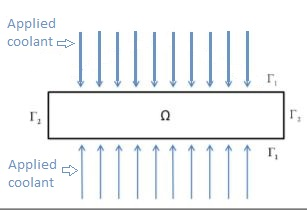
\includegraphics{figures/steel_slab_visualization.jpg}
    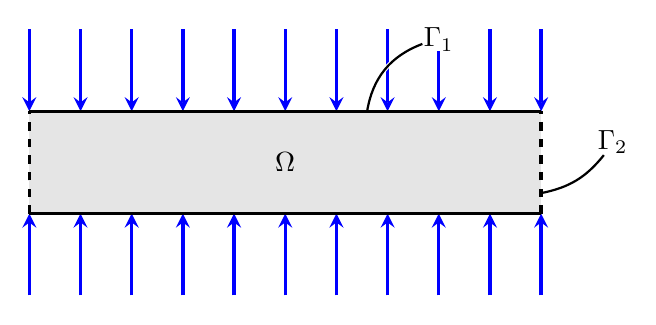
\begin{tikzpicture}[very thick, >=stealth, scale=1.3]
\draw (0, 0) -- (5, 0);
\draw (0, 1) -- (5, 1);
\draw[dashed] (0, 0) -- (0, 1);
\draw[dashed] (5, 0) -- (5, 1);
\node (domain) at (2.5, .5) {$\Omega$};
\foreach \x in {0, 0.5, ..., 5} {
    \draw[->, color=blue] (\x, -.8) -- (\x, 0);
    \draw[->, color=blue] (\x, 1.8) -- (\x, 1);
}
\node[fill=white, inner sep=0] (gamma1-1) at (4, 1.7) {$\Gamma_1$};
\node[fill=white, inner sep=0] (gamma2-1) at (5.7, 0.7) {$\Gamma_2$};
\draw[ultra thick, color=white] (gamma1-1) to [bend right=30] (3.3, 1);
\draw[thick] (gamma1-1) to [bend right=30] (3.3, 1);
\draw[thick] (gamma2-1) to [bend left=20] (5, 0.2);
\fill[black!10] (0, 0) rectangle (5, 1);
\draw (0, 0) -- (5, 0);
\draw (0, 1) -- (5, 1);
\draw[dashed] (0, 0) -- (0, 1);
\draw[dashed] (5, 0) -- (5, 1);
\node (domain) at (2.5, .5) {$\Omega$};
\end{tikzpicture}
    \caption{An illustration of our steel slab where we have shown the applied cooling, we have isolation on $\Sigma_2$ by the optimal control problem \eqref{eq:heat}}
    \label{fig:steel_slab}
\end{figure}

In the case of dual phase steel we can consider a more realistic scenario used in the industry. To do so we introduce two desired temperatures $\theta_{d_1}$ and $\theta_{d_2}$. For the optimal cooling of dual phase steel there is a phase transition in the higher temperature regime, this is modelled by the desired temperature $\theta_{d_1}$ which we want to be attained in a subset $[c_1T, c_2T]$ of $[0,T]$ with $c_2 <1$. Then we expect the optimal cooling to lead to a rapid cooling towards $\theta_{d_1}$ and stay almost constant until $t=c_2T$. Then we also expect the optimal cooling strategy to lead to a rapid cooling towards the new final desired temperature $\theta_{d_2}$. In order to model this scenario we need to introduce an extra term to the cost functional. Consequently we will get a new adjoint system, however the expression for the gradient stays the same, as the new term does not involve the control, so we can apply the Projected gradient method in Algorithm 1 almost without doing any modifications. The new cost functional is given by 

\begin{equation}
    \label{eq:new_cost}
    J(\theta,u) : = \frac{\alpha_1}{2}\iint_{Q}\chi_{[c_1T,c_2T]}(\theta(x,t) - \theta_{d_1}(x,t))^2 \dxdt + \frac{\alpha_2}{2}\int_{\Omega} (\theta(x,T) - \theta_{d_2})^2 \dxdt + \frac{\gamma}{2}\int_0^T|u(t)|^2\dt
\end{equation}

Here $\chi_E$ denotes the characteristic function for the set $E$. For convenience we formulate the whole optimal control problem in this case. 

\begin{align*}
       \min J(\theta, u) = \frac{\alpha_1}{2}\iint_{Q}\chi_{[c_1T,c_2T]}(\theta(x,t) - \theta_{d_1}(x,t))^2 \dxdt + \frac{\alpha_2}{2} \int_\Omega (\theta(x, T) - \theta_d)^2 \mathop{dx} \mathop{dt} + \frac{\gamma}{2} \int_0^{T} u^2 \mathop{dt} \\
       \text{subject to} \\
       \rho c_p \theta_t - \nabla \cdot (k \nabla \theta) &= 0 \quad &\text{in } Q  \\
      -k \frac{\partial \theta}{\partial \nu} &= u(t) (\theta - \theta_w) \quad &\text{on } \Sigma_1, \\
      -k \frac{\partial \theta}{\partial \nu} &= 0 \quad &\text{on } \Sigma_0, \\
      \theta(x, 0) &= \theta_0 &
\end{align*}

We again use the formal Lagrange method to derive the adjoint system. The lagrangian takes the same form except an additional term which gives an extra contribution to the adjoint system. Taking the Frechet derivative with respect to the state of the Lagrangian we get

\begin{equation}
  \begin{aligned}
  0 = \L_\theta(\theta, u, p)h = \alpha_2 \int_\Omega (\theta(x,T) - \theta_d)h(x, T)\dx - \iint_Q h_t p\dxdt \\
  - \frac{k}{\rho c_p}\iint_Q\nabla h\nabla p \dxdt
  - \frac{1}{\rho c_p}\iint_{\Sigma_1} u(t)h p\dsdt \\
  + \alpha_1 \iint_{Q}\chi_{[c_1T,c_2T]}(\theta - \theta_{d_1})h \dxdt
  \end{aligned}
\end{equation}